\chapter{Conclusions}

\section{Conclusions}

In this work, we introduced a method that leverages self-supervised deep neural networks to learn low-dimensional music latent representations with applications to music boundary detection. Building on existing approaches and architectures, we replaced traditional features with deep embeddings trained to represent high-level musical information to analyze its performance in music segmentation tasks.

While our musically-informed technique does not yet outperform the existing state-of-the-art baselines \cite{deepfeaturesegment, SalamonDeepSegmentation}, it exhibits significant potential in boundary detection tasks, particularly when expanding the training set. The improvement we've observed between datasets is noteworthy, and when compared with two of the acoustic features, our results are highly competitive. We've also managed to circumvent the typical issues associated with dataset enlargements, such as the need for extensive supervision or human annotation, which gives our method an edge in terms of practicality and scalability, effectively turning what is usually seen as an expensive hurdle into a much more manageable task.

\section{Discussion}

Whether our model effectively decodes underlying high-level musical content remains open to scientific investigation. It's plausible that our technique possesses significant potential for nearly all content-based MIR downstream tasks, given its intention to be both sound-agnostic and content-sensitive. Queries persist about whether such a general-purpose audio representation can mimic human hearing \cite{Li2023MERT:Training, Turian2022HEAR:Representations}, or if it can accurately decode high-level musical content. Such questions remain unresolved due to the current lack of evaluative measures. 

This represents a 'thorn in our side' that we intend to address in future research.

We argue whether factors such as the size of the representation layer and the size of the model \cite{verydeep} might be insufficient. Furthermore, we posit that with additional time to iterate repeatedly over the dataset, the loss function could decrease further with minimal risk of overfitting. \ref{fig:lossf}

While our results may not yet rival state-of-the-art benchmarks, they affirm we're on the right path and reveal the potential of this research direction. Importantly, we've seen that progress doesn't have to be expensive—though time and potential copyright issues are considerations.

\begin{figure}[h]
    \centering
    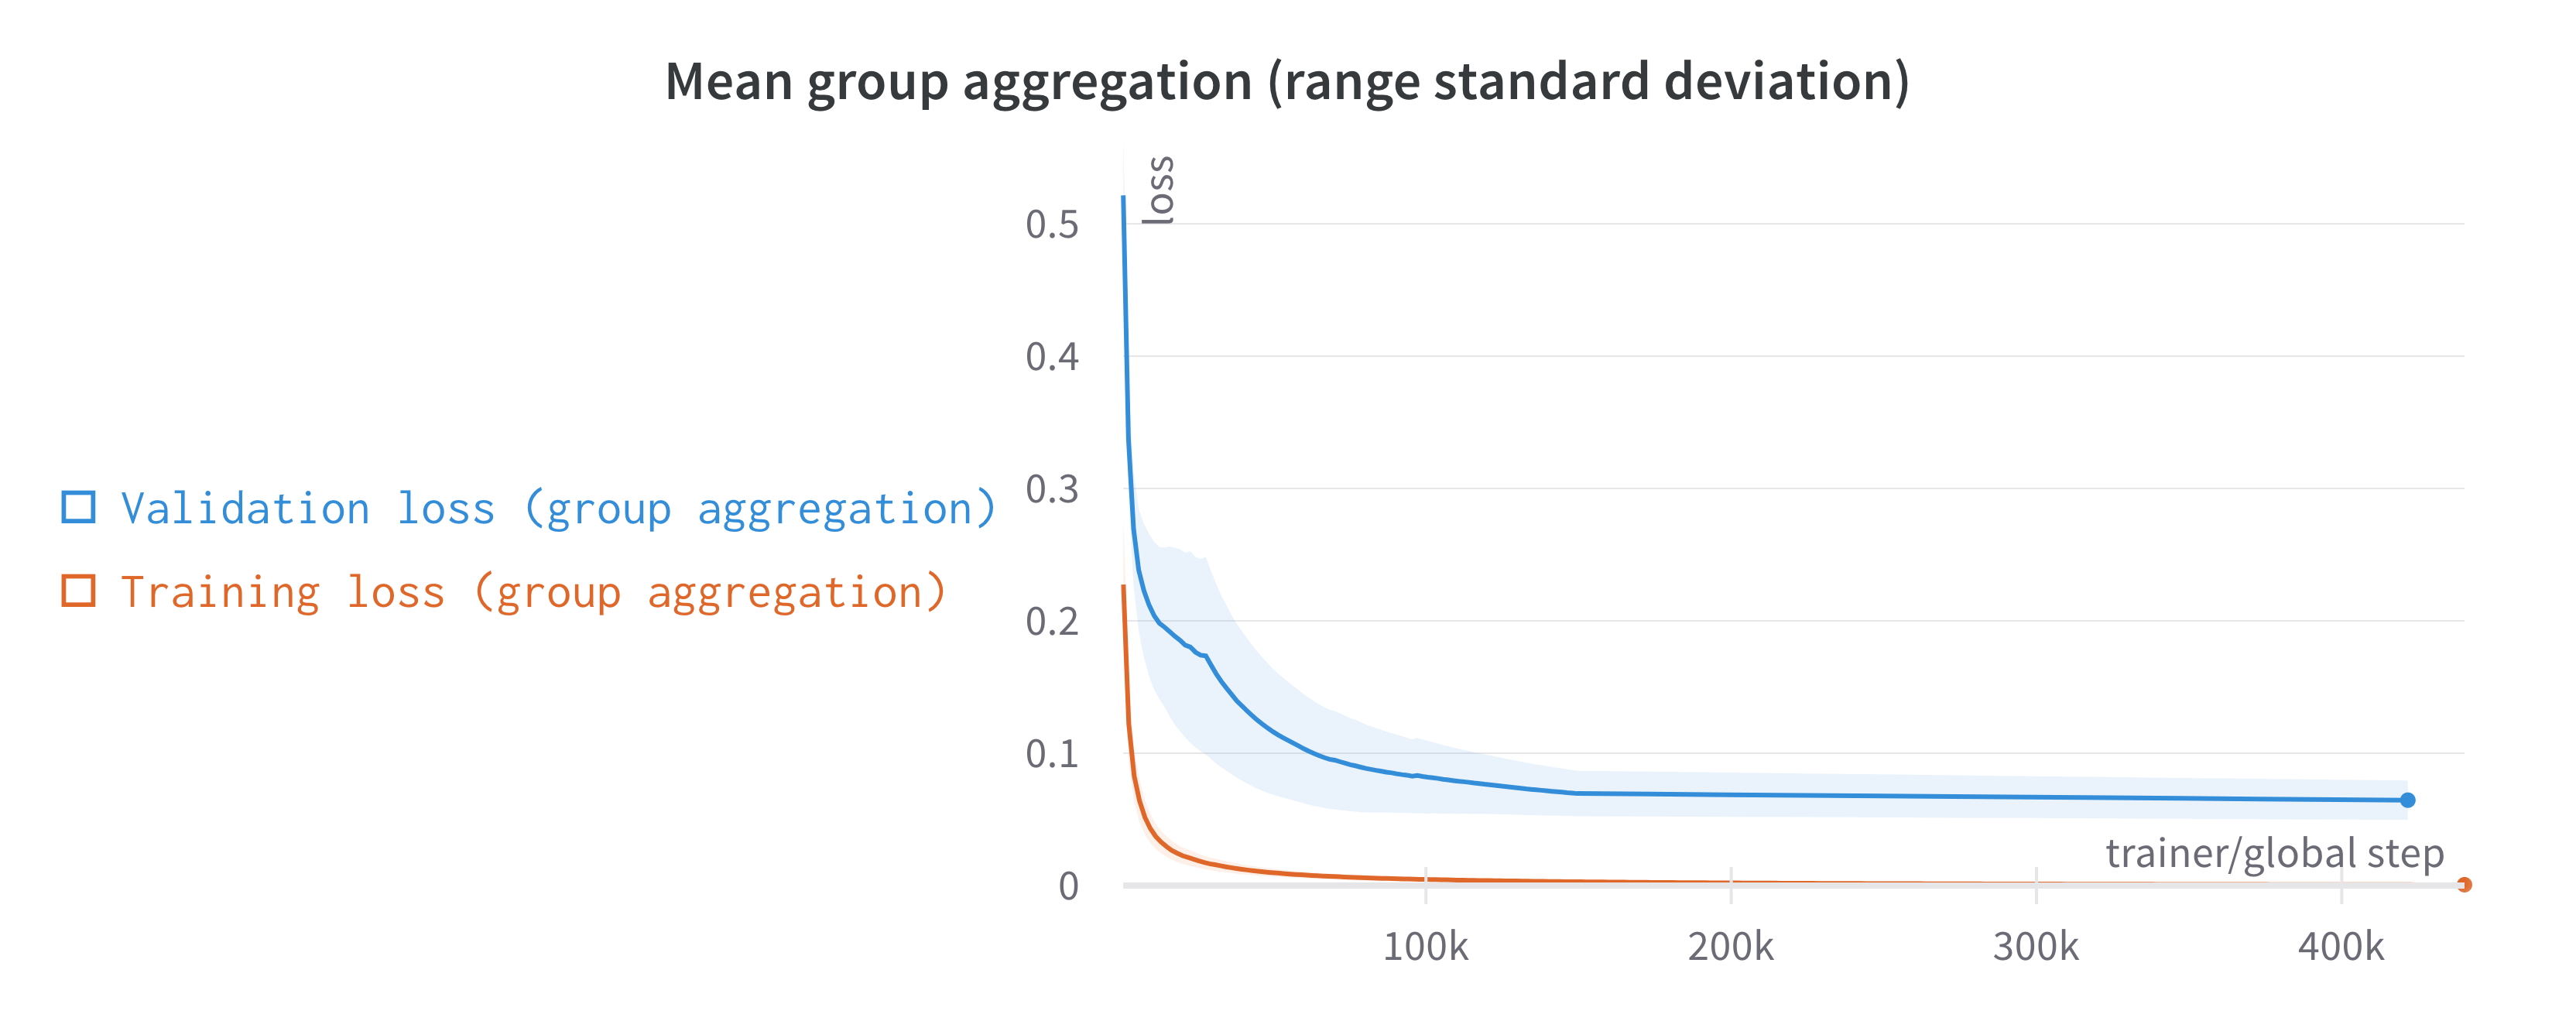
\includegraphics[width=\textwidth]{figures/images/Mean group aggregation.png}
    \caption[Loss function performance plot]{Mean group aggregation of the decrease of the loss function over trainer/global steps. Training loss against validation loss.}
    \label{fig:lossf}
\end{figure}



\newpage


